% Created 2024-07-08 Mon 22:16
% Intended LaTeX compiler: pdflatex
\documentclass[11pt]{article}
\usepackage[utf8]{inputenc}
\usepackage[T1]{fontenc}
\usepackage{ragged2e}
\usepackage{caladea}
\usepackage{graphicx}
\usepackage{longtable}
\usepackage{wrapfig}
\usepackage{rotating}
\usepackage{epigraph}
\usepackage[normalem]{ulem}
\usepackage{hyperref}
\usepackage{amsmath}
\usepackage{amssymb}
\usepackage{capt-of}
\usepackage{hyperref}
\usepackage{fancyhdr}
\title{Novena à Santa Bibiana}
 % \hypersetup{
 %  pdfauthor={},
 %  pdftitle={Novena a/à SANTO_NOME},
 %  pdfkeywords={},
 %  pdfsubject={},
 %  pdfcreator={Emacs 29.4 (Org mode 9.6.15)}, 
 %  pdflang={English}
 % }

\title{
  \par
  NOVENA À SÃO FRANCISCO DE SÃO MIGUEL}
\author{Garamog, Nina Freitas}
\date{30/11 - 08/12}
\renewcommand{\contentsname}{Sumário}

\begin{document}


\maketitle
\thispagestyle{empty}

\pagestyle{fancy}
\fancyhf{} % clear existing header/footer entries
\fancyfoot[LO, CE]{
  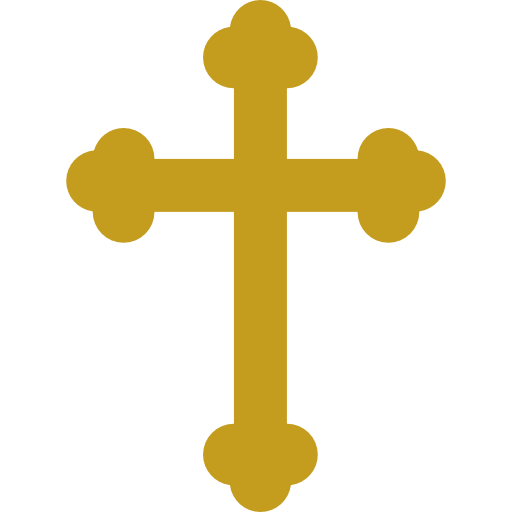
\includegraphics[scale=0.2]{./assets/cross.png} São Francisco de São Miguel, Rogai por Nós!
}
% Place Page X of Y on the right-hand
% side of the footer
\fancyfoot[R]{\thepage}
  
\newpage

\tableofcontents

\centering
\vfill
Visite-nos no Telegram: \url{https://t.me/CotidieNovena}
\newpage




%%%%%%%%%%%%%%%%%%%%%%%%%%%%%%%%%%%%% História  %%%%%%%%%%%%%%%%%%%%%%%%%%%%%%%%%%%%%%%%%%%
\section{História}\label{historia}

\begin{justify}

\subsection {Mártir no Japão, religioso da Primeira Ordem (1543-1597). Canonizado por Pio IX em 8 de junho de 1862.}

Nasceu na Diocese de Palência, na Espanha, em 1543, de uma família profundamente religiosa. Desde pequeno se distinguiu pela piedade, modéstia, pureza e amor à oração.

Em 1556 vestiu o hábito de São Francisco, na Ordem dos Frades Menores. Em sua humildade preferiu ser irmão, feliz de poder se dedicar aos serviços da casa, exercendo-os com alegria.

Desejoso de maior austeridade, pediu para ser admitido na Província de São José, fundado pelo asceta São Pedro de Alcântara. Teve uma grande sede do martírio e de dedicar sua vida à obra da evangelização. Foi designado como companheiro de São Pedro Batista para a viagem ao México e Filipinas. Na sua última missão, mesmo não sendo sacerdote, recebeu a tarefa de pregar o evangelho na Província das Ilhas Canárias, onde pela palavra, confirmou grandes prodígios, desencadeando inúmeras conversões.

No Japão, trabalhou muito pela conversão dos japoneses. Em 9 de dezembro de 1596 foi detido em Osaka e mudado para Meaco, onde teve a sua orelha esquerda cortada. Junto com os seus companheiros em Nagasaki, foi crucificado. Tinha 54 anos de idade. A execução do martírio foi presenciado por inúmeros cristãos e marinheiros portugueses.


\end{justify}

\subsection*{Créditos }
\href{https://franciscanos.org.br/carisma/calendario/sao-francisco-de-sao-miguel#gsc.tab=0}{Província Franciscana da Imaculada Conceição do Brasil}

\newpage


%%%%%%%%%%%%%%%%%%%%%%%%%%%%%%%%%%%%% Orações  %%%%%%%%%%%%%%%%%%%%%%%%%%%%%%%%%%%%%%%%%%%
\section{Orações}\label{oracoes}

\subsection{Oração para todos os dias:} \label{oracao-canonizacao}

Ó São Francisco de São Miguel, vós que, desejoso de maior austeridade, pediste para ser admitido na província de São José, fundada pelo venerável São Pedro de Alcântara, e tiveste uma grande sede do martírio e de dedicar a vossa vida à obra da evangelização, dai-nos a graça que necessitamos nesta novena e, principalmente, a graça de sermos cada dia mais fiéis a Deus.

[Peça a sua graça aqui.]

\textbf{Pai-Nosso, Avé-Maria e Glória.}

\subsection*{Créditos:}
\href{https://www.youtube.com/watch?v=5uurRmRqG_U&list=PLRL6i6PPLb59lYAov5lt4llBN4eevfdkR}{Canal Virtude Plena - YouTube}


\end{document}
